\documentclass[12pt,]{article}
\usepackage{lmodern}
\usepackage{amssymb,amsmath}
\usepackage{ifxetex,ifluatex}
\usepackage{fixltx2e} % provides \textsubscript
\ifnum 0\ifxetex 1\fi\ifluatex 1\fi=0 % if pdftex
  \usepackage[T1]{fontenc}
  \usepackage[utf8]{inputenc}
\else % if luatex or xelatex
  \ifxetex
    \usepackage{mathspec}
    \usepackage{xltxtra,xunicode}
  \else
    \usepackage{fontspec}
  \fi
  \defaultfontfeatures{Mapping=tex-text,Scale=MatchLowercase}
  \newcommand{\euro}{€}
\fi
% use upquote if available, for straight quotes in verbatim environments
\IfFileExists{upquote.sty}{\usepackage{upquote}}{}
% use microtype if available
\IfFileExists{microtype.sty}{%
\usepackage{microtype}
\UseMicrotypeSet[protrusion]{basicmath} % disable protrusion for tt fonts
}{}
\usepackage[margin=1in]{geometry}
\ifxetex
  \usepackage[setpagesize=false, % page size defined by xetex
              unicode=false, % unicode breaks when used with xetex
              xetex]{hyperref}
\else
  \usepackage[unicode=true]{hyperref}
\fi
\hypersetup{breaklinks=true,
            bookmarks=true,
            pdfauthor={},
            pdftitle={},
            colorlinks=true,
            citecolor=blue,
            urlcolor=black,
            linkcolor=black,
            pdfborder={0 0 0}}
\urlstyle{same}  % don't use monospace font for urls
\setlength{\parindent}{0pt}
\setlength{\parskip}{6pt plus 2pt minus 1pt}
\setlength{\emergencystretch}{3em}  % prevent overfull lines
\setcounter{secnumdepth}{0}

%%% Use protect on footnotes to avoid problems with footnotes in titles
\let\rmarkdownfootnote\footnote%
\def\footnote{\protect\rmarkdownfootnote}

%%% Change title format to be more compact
\usepackage{titling}

% Create subtitle command for use in maketitle
\newcommand{\subtitle}[1]{
  \posttitle{
    \begin{center}\large#1\end{center}
    }
}

\setlength{\droptitle}{-2em}
  \title{}
  \pretitle{\vspace{\droptitle}}
  \posttitle{}
  \author{}
  \preauthor{}\postauthor{}
  \date{}
  \predate{}\postdate{}

\usepackage{lineno}
\linenumbers
\usepackage{setspace}
\usepackage{todonotes}
\usepackage{color}
\usepackage{rotating}
\usepackage{morefloats}


\begin{document}

\maketitle


\begin{center} 
\textbf{ONLINE SUPPORTING INFORMATION}
\end{center}

\renewcommand{\theequation}{S\arabic{equation}}
\renewcommand{\thetable}{S\arabic{table}}
\renewcommand{\thefigure}{S\arabic{figure}}

\tableofcontents
\listoffigures
\listoftables
\newpage{}

\subsection{Derivation of limiting case predictions for synchrony of per
capita growth rates (Equations
3-4)}\label{derivation-of-limiting-case-predictions-for-synchrony-of-per-capita-growth-rates-equations-3-4}

Following Loreau and {{de Mazancourt}} (2013) and {{de Mazancourt}} et
al. (2013), we define population growth, ignoring observation error, as

\begin{align}
r_i(t) = r_{mi} \left[ 1- \frac{N_i(t)+\sum_{j \neq i} \alpha_{ij}N_j(t)} {K_i} + \sigma_{ei}u_{ei}(t) + \frac{\sigma_{di}u_{di}(t)}{\sqrt{N_i(t)}} \right]
\end{align}

\noindent where \(N_i(t)\) is the biomass of species \emph{i} in year
\emph{t}, and \(r_i(t)\) is its growth rate in year \emph{t}. \(r_{mi}\)
is species \emph{i}'s intrinsic rate of increase, \(K_i\) is its
carrying capacity, and \(\alpha_{ij}\) is the interspecific competition
coefficient representing the effect of species \emph{j} on species
\emph{i}. Environmental stochasticity is incorporated as
\(\sigma_{ei}u_{ei}(t)\), where \(\sigma_{ei}^2\) is the environmental
variance and \(u_{ei}\) are normal random variables with zero mean and
unit variance that are independent through time but may be correlated
between species. Demographic stochasticity arises from variations in
births and deaths among individuals (e.g., same states, different
fates), and is included in the model as a first order, normal
approximation (Lande et al. 2003, {{de Mazancourt}} et al. 2013).
\(\sigma_{di}^2\) is the demographic variance and \(u_{di}(t)\) are
independent normal variables with zero mean and unit variance.

First-order approximations of the temporal variance of total community
biomass are obtained as follows (Ives 1995, Hughes and Roughgarden 2000,
Ives and Hughes 2002, Loreau and {{de Mazancourt}} 2008, {{de
Mazancourt}} et al. 2013). Let \(\delta N_i(t) = N_i(t) - N^*_i\) denote
the deviation of observed species \emph{i}'s biomass from its
equilibrium value in the community, \(N^*_i\), in the absence of
stochasticity. Equation (S1) can be Taylor expanded around
\(\delta N_i(t) = u_{ei}(t) = u_{di}(t) = u^S_{oi}(t) = 0\) to yield,
after dropping terms of order two and higher,

\begin{equation}
\boldsymbol{\delta}\textbf{N}(t+1) = \textbf{A}\boldsymbol{\delta}\textbf{N}(t) + \textbf{z}(t),
\end{equation}

\noindent where \(\boldsymbol{\delta}\textbf{N}(t)\) is the vector of
deviations of species biomasses from their deterministic equilibrium
value, \textbf{A} is the community matrix, also known as the Jacobian
matrix around the equilibrium, with elements \((a_{ij})_{1<i,j<S}\):

\begin{align}
A_{ij} = 
  \begin{cases}
      1-r_{mi} \frac{N_{i}^*}{K_i}, & i=j \\
      -r_{mi} \frac{N_{i}^*}{K_i} \alpha_{ij}, & i \neq j
    \end{cases}
\end{align}

\noindent and \(\textbf{z}(t)\) is a vector that encapsulates the
effects of environmental and demographic stochasticity whose elements
are

\begin{equation}
z_i(t) = N^*_i \sigma_{ei} u_{ei}(t) + \sqrt{N^*_i} \sigma_{di} u_{di}(t)
\end{equation}

When the system reaches a stationary distribution, the variances and
covariances between species biomass time series are:

\begin{equation}
\big\langle \boldsymbol{\delta}\textbf{N}(t) \boldsymbol{\delta}\textbf{N}(t)^T \big\rangle = \textbf{C}^\infty = (\text{cov}(N_i,N_j))_{1<i,j<S} = (\text{cov}(\delta N_i, \delta N_j))_{1<i,j<S}
\end{equation}

\noindent where \(\boldsymbol{\delta}\textbf{N}^T\) is the transpose of
vector \(\boldsymbol{\delta}\textbf{N}\), i.e.~a row vector.

Our assumptions listed above lead to the following correlation structure
of \textbf{z}:

\begin{equation}
\big\langle \textbf{z}(t) \textbf{z}(t)^T \big\rangle = \textbf{B}
\end{equation}

\begin{equation}
\big\langle \textbf{z}(t-s) \textbf{z}(t)^T \big\rangle = 0 \qquad \text{for} \: s>0
\end{equation}

We use Equation S2 to write a dynamical equation for the covariance
\textbf{C}:

\begin{footnotesize}
\begin{align}
\textbf{C}(t+1) =& \big\langle \boldsymbol{\delta}\textbf{N}(t+1) \boldsymbol{\delta}\textbf{N}(t+1)^T \big\rangle \\
=& \textbf{A}\big\langle \boldsymbol{\delta}\textbf{N}(t) \boldsymbol{\delta}\textbf{N}(t)^T \big\rangle \textbf{A}^T + \textbf{A}\big\langle \boldsymbol{\delta}\textbf{N}(t) \boldsymbol{\delta}\textbf{N}(t)^T \big\rangle + \big\langle \textbf{z}(t) \boldsymbol{\delta}\textbf{N}(t)^T \big\rangle \textbf{A}^T + \big\langle \textbf{z}(t) \textbf{z}(t)^T \big\rangle \\
=& \textbf{A} \textbf{C}(t) \textbf{A}^T + \textbf{Z}_0
\end{align}
\end{footnotesize}

\noindent Taking the limit \(t \rightarrow \infty\) on both sides, we
get:

\begin{equation}
\textbf{C}^\infty = \textbf{A} \textbf{C}^\infty \textbf{A}^T + \textbf{B}
\end{equation}

\noindent where \textbf{A} is as in Equation S3 and \textbf{B} is:

\begin{equation}
B_{ij} = N_{i}^* N_{j}^* \sigma_{ei} \sigma_{ej} \text{cov}(u_{ei},u_{ej}) + \sqrt{N_{i}^* N_{j}^*} \sigma_{di}\sigma_{dj} \text{cov}(u_{di},u_{dj})
\end{equation}

\noindent Similarly, \textbf{R} is the variance-covariance matrix for
population growth rates at steady state

\begin{equation}
R_{ij} = \frac{r_{mi}r_{mj}}{K_i K_j} \sum_{k,l} \alpha_{ik} \alpha_{jl} C_{kl} + \sigma_{ei} \sigma_{ej} \text{cov}(u_{ei},u_{ej}) + \frac{\sigma_{di}\sigma_{dj} \text{cov}(u_{di},u_{dj})}{\sqrt{N_{i}^* N_{j}^*}}.
\end{equation}

\noindent Then, following the synchrony metric of Loreau and {{de
Mazancourt}} (2008), the sychrony of population biomasses is

\begin{equation}
\phi_N = \frac{\sum_{i,j}C_{ij}}{\left( \sum_i \sqrt{C_{ii}} \right)^2}
\end{equation}

\noindent and the synchrony of per capita growth rates is

\begin{equation}
\phi_R = \frac{\sum_{i,j}R_{ij}}{\left( \sum_i \sqrt{R_{ii}} \right)^2}.
\end{equation}

Synchrony of population biomasses and growth rates emerge from complex
interactions among species' intrinsic growth rates, interspecific
interactions, environmental stochasticity, and demographic
stochasticity. Given these complexities, it is impossible to determine
expected effects of different parameters in a multi-species case. Thus,
we analyze a simplified case where interspecific interactions are zero.
The variance-covariance matrix of population biomasses at steady state
then becomes

\begin{equation}
c_{ij} = \frac{B_{ij}}{1-A_ii A_jj} = \frac{N_{i}^* N_{j}^* \sigma_{ei} \sigma_{ej} \text{cov}(u_{ei},u_{ej}) + \sqrt{N_{i}^* N_{j}^*} \sigma_{di}\sigma_{dj} \text{cov}(u_{di},u_{dj})}{1 - (1-r_{mi})(1-r_{mj})}
\end{equation}

and the variance-covariance matrix of population growth rates simplifies
to

\begin{equation}
R_{ij} = \frac{1}{1- \frac{r_{mi}r_{mj}}{r_{mi}+r_{mj}}} \left( \sigma_{ei} \sigma_{ej} \text{cov}(u_{ei},u_{ej}) + \frac{\sigma_{di}\sigma_{dj} \text{cov}(u_{di},u_{dj})}{\sqrt{N_{i}^* N_{j}^*}} \right)
\end{equation}

\noindent Note that synchrony in population sizes and synchrony in
growth rates use weighted factors of the environmental variances and
covariances with species-specific parameters. So, we further assume
that, along with interspecific interactions being zero, all species have
identical growth rates, environmental stochasticity is absent, and all
species have identical demographic variance. This represents a
theoretical limiting case where the community consists of identical
species coexisting in a constant environment where only demographic
stochasticity causes temporal fluctuations. Under such conditions,
synchrony of population biomasses is

\begin{equation}
\phi_N = \frac{1}{\left(\sum_i p_i^{1/2} \right)^2}
\end{equation}

\noindent and synchrony of growth rates is

\begin{equation}
\phi_R = \frac{\sum_i p_i^{-1}}{\left(\sum_i p_i^{-1/2} \right)^2}
\end{equation}

\noindent where \(p_i\) is the average frequency of species \emph{i},
\(p_i = N_i/N_T\). When all species have identical abundances and
\(p_i = 1/S\), where \emph{S} is species richness, the both synchrony
values equal 1/S (Loreau and {{de Mazancourt}} 2008). The prediction
represented in Equation S19 is Equation 3 in the main text, which we
refer to as \(\phi_{R,\mathcal{M}_D}\).

Another limiting case is where only environmental stochasticity is
operating: no interspecific interactions, no demographic stochasticity,
identical intrinsic growth rates, and environmental stochasticity with
same standard deviation for all species. Under such constraints, the
synchrony of of species' biomasses is

\begin{equation}
\phi_N = \sum_{i,j} p_i p_j \text{cov}(u_{ei}, u_{ej})
\end{equation}

\noindent{} and the synchrony of species' growth rates is

\begin{equation}
\phi_R = \frac{\sum_{i,j} \text{cov}(u_{ei}, u_{ej})}{S^2}
\end{equation}

\noindent The prediction represented in Equation S21 is Equation 4 in
the main text, which we refer to as \(\phi_{R,\mathcal{M}_E}\). If we
know the covariance matrix of the species environmental responses, we
can calculate the above expectations directly. Note that the
environmental responses are normalized in the above equations, therefore
the covariances are correlations in the above equations.

\newpage{}

\subsection{Materials and methods
details}\label{materials-and-methods-details}

\subsubsection{Vital rate statistical
models}\label{vital-rate-statistical-models}

We modeled survival probability and growth on individual genets as a
function of genet size, the crowding experienced by the focal genet from
both heterospecific and conspecific genets in its neighborhood
(described below), temporal varation among years, and spatial variation
among quadrat groups. Groups are sets of quadrats located in close
proximity within a pasture or grazing exclosure.

We follow the approach of Chu and Adler (2015) to estimate crowding,
assuming that the crowding experienced by a focal genet depends on
distance to each neighbor genet and the neighbor's size, \emph{u}:

\begin{equation}
w_{ijm,t} = \sum_k e^{-\delta_{jm}d_{ijkm,t}^{2}}u_{km,t}.
\end{equation}

In the above, \(w_{ijm,t}\) is the crowding that genet \emph{i} of
species \emph{j} in year \emph{t} experiences from neighbors of species
\emph{m}. The spatial scale over which species \emph{m} neighbors exert
influence on any genet of species \emph{j} is determined by
\(\delta_{jm}\). The function is applied for all \emph{k} genets of
species \emph{m} that neighbor the focal genet at time \emph{t}, and
\(d_{ijkm,t}\) is the distance between genet \emph{i} in species
\emph{j} and genet \emph{k} in species \emph{m}. When \(k=m\), the
effect is intraspecific crowding. We use regression-specific (survival
and growth) \(\delta\) values estimated by Chu and Adler (2015).

We used logistic regression to model survival probability (\(S\)) of
genet \(i\) from species \(j\) in quadrat group \(g\) from time \(t\) to
\(t+1\):

\begin{align}
\text{logit}(S_{ijg,t}) &= \gamma^{S}_{j,t} + \phi^{S}_{jg} + \beta^{S}_{j,t}x_{ij,t} + \boldsymbol{\omega}^{S}_{j} \textbf{w}_{ij,t}
\end{align}

where \(x_{ij,t}\) is the log of genet size, \(\gamma^{S}_{j,t}\) is a
year-specific intercept, \(\beta^{S}_{j,t}\) is the year-specific slope
parameter for size, \(\phi^{S}_{jg}\) is the random effect of quadrat
group location, and \(\omega\) is a vector of per capita interaction
coefficients which determine the impact of crowding, \textbf{w}, by each
species on the focal species.

We modeled genet growth, conditional on survival, in a similar manner:

\begin{align}
\mu_{ijg,t+1} &= \gamma^{G}_{j,t} + \phi^{G}_{jg} + \beta^{G}_{j,t}\mu_{ij,t} + \boldsymbol{\omega}^{G}_{j} \textbf{w}_{ij,t}
\end{align}

where \(\mu\) is log genet size and all other parameters are as
described for the survival regression. We capture non-constant error
variance in growth by modeling the variance around the growth regression
(\(\varepsilon\)) as a nonlinear function of predicted genet size:

\begin{align}
\varepsilon_{ij,t} = a e^{b \mu_{ijg,t+1}}
\end{align}

Our data allows us to track new recruits, but we cannot assign a
specific parent to new genets. THerefore, we model recruitment at the
quadrat level: the number of new individuals of species \(j\) in quadrat
\(q\) recruiting at time \(t+1\) as a function of quadrat ``effective
cover'' (\(A'\)) in the previous year (\(t\)). Effective cover is a
mixture of observed cover (\(A\)) in the focal quadrat (\(q\)) and the
mean cover across the entire group (\(\bar{A}\)) of \(Q\) quadrats in
which \(q\) is located:

\begin{equation}
A'_{jq,t} = p_{j}A_{jq,t} + (1-p_{j})\bar{A}_{jQ,t}
\end{equation}

where \(p\) is a mixing fraction between 0 and 1 that is estimated
within the model.

We assume the number of individuals, \(y^{R}\), recruiting at time
\(t+1\) follows a negative binomial distribution:

\begin{equation}
y^{R}_{jq,t+1} \sim \text{NegBin}(\lambda_{jq,t+1},\zeta)
\end{equation}

where \(\lambda\) is the mean intensity and \(\zeta\) is the size
parameter. We define \(\lambda\) as:

\begin{equation}
\lambda_{jq,t+1} = A'_{jq,t}e^{(\gamma^{R}_{j,t} + \phi^{R}_{jQ} + \theta^{R}_{jk}C_{k,t} + \omega^{R}\sqrt{A'_{q,t}})}
\end{equation}

where \(A'\) is effective cover (\(\text{cm}^2\)) of species \(j\) in
quadrat \(q\) and all other terms are as in the survival and growth
regressions.

\subsubsection{Multi-species populations
models}\label{multi-species-populations-models}

The individually based model (IBM) is straighforward and described in
the main text, so here focus on the structure of the integral projeciton
model (IPM). We built an environmentally stochastic IPM. Our IPM follows
the specification of Chu and Adler (2015) where the population of
species \emph{j} is a density function \(n(u_{j},t)\) giving the density
of sized-\emph{u} genets at time \emph{t}. Genet size is on the natural
log scale, so that \(n(u_{j},t)du\) is the number of genets whose area
(on the arithmetic scale) is between \(e^{u_{j}}\) and \(e^{u_{j}+du}\).
So, the density function for any size \emph{v} at time \(t+1\) is

\begin{equation}
n(v_{j},t+1) = \int_{L_{j}}^{U_{j}} k_{j}(v_{j},u_{j},\bar{\bold{w_{j}}}(u_{j}))n(u_{j},t)
\end{equation}

where \(k_{j}(v_{j},u_{j},\bar{\bold{w_{j}}})\) is the population kernal
that describes all possible transitions from size \(u\) to \(v\) and
\(\bar{\bold{w_{j}}}\) is a vector of estimates of average crowding
experienced from all other species by a genet of size \(u_j\) and
species \(j\). The integral is evaluated over all possible sizes between
predefined lower (\emph{L}) and upper (\emph{U}) size limits that extend
beyond the range of observed genet sizes.

The population kernal is defined as the joint contributions of survival
(\emph{S}), growth (\emph{G}), and recruitment (\emph{R}):

\begin{equation}
k_{j}(v_{j},u_{j},\bar{\bold{w_{j}}}) = S_j(u_j, \bar{\bold{w_{j}}}(u_{j}))G_j(v_{j},u_{j},\bar{\bold{w_{j}}}(u_{j})) + R_j(v_{j},u_{j},\bar{\bold{w_{j}}}),
\end{equation}

\noindent{} which means we are calculating growth (\emph{G}) for
individuals that survive (\emph{S}) from time \emph{t} to \emph{t+1} and
adding in newly recruited (\emph{R}) individuals of an average sized
one-year-old genet for the focal species. Our stastical model for
recruitment (\emph{R}, described below) returns the number of new
recruit produced per quadrat. Following previous work, we assume that
fecundity increases linearly with size
(\(R_j(v_{j},u_{j},\bar{\bold{w_{j}}}) = e^{u_j}R_j(v_{j},\bar{\bold{w_{j}}})\))
to incorporate the recruitment function in the spatially-implicit IPM.

\newpage{}

\subsection{Results for synchrony of percent
cover}\label{results-for-synchrony-of-percent-cover}

Synchrony of percent cover from population model simulations did not
compare well with observed synchrony of cover or analytical predictions
for synchrony cover (Fig. S2, S3). We did not expect synchrony of
percent cover from simulations to compare well with observed synchrony
of cover because our models represent equilibrium dynamics rather than a
specific set of observed years. Also, unlike growth rates, synchrony in
cover is highly influenced by drift and legacy effects (Loreau and {{de
Mazancourt}} 2008).

More interesting is that our simulation results did not compare well
with analytical predictions. One issue is that some species are not
well-regulated around their equilibrium cover, so that our linear
approximation required for anayltical predictions is likely to fail.
Analytical predictions for synchrony of growth rates are more
informative than synchrony in population sizes because the linear
approximation is more proximate.

Another issue is the influence of demographic stochasticity in some
communities, for example, in Idaho where our simulations with only
demographic stochasticity yielded results far different from analytical
predicitons (Fig. S2). Our analytical predictions require the
unrealistic assumption that demographic variances among species are
equal. However, in Idaho, \emph{A. tripartita} has much higher
demographic stochasticity than the other species, so that variation in
its abundance dominates. Thus, the assumption that all species have
similar stochasticity fails. In combination, our results from analyzing
synchrony of percent cover indicate that the best way to decipher the
mechanisms contributing to community synchrony is to analyze growth
rates, in agreement with the theoretical arguments of Loreau and {{de
Mazancourt}} (2008).

\newpage{}

\subsection{Supporting Figures}\label{supporting-figures}

\begin{figure}[!ht]
  \centering
      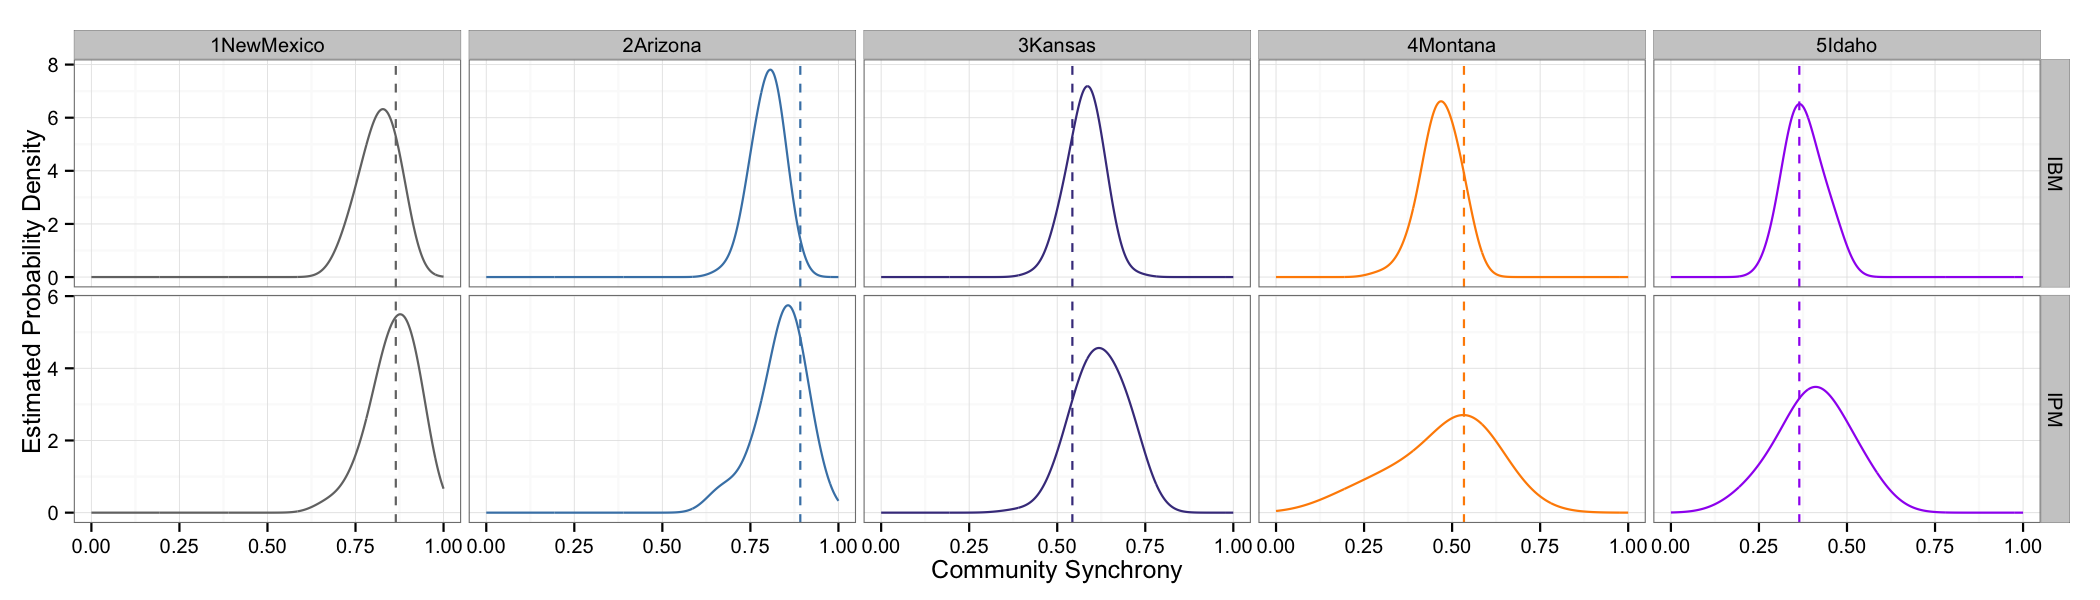
\includegraphics[width=6in]{./components/figureS1.png}
  \caption{Observed (vertical dashed lines) and simulated (solid density curves) synchrony of species per capita growth rates at each site from the IBM (top panels) and the IPM (bottom panels). IPM density curves come from 100 random contiguous sections from 2,000 iteration IPM runs, where the length of each randomly selected section is equal to the numnber of observation years for each data set. IBM density curves come from 100 replicate simulations of 75 iterations each. Synchrony values come from simulations where environmental stochasticity and interspecific interactions are present. The IBM was run on a 5 by 5 meter landscape to reduce the effect of demographic stochasticity.}
\end{figure}

\pagebreak{}

\begin{figure}[!ht]
  \centering
      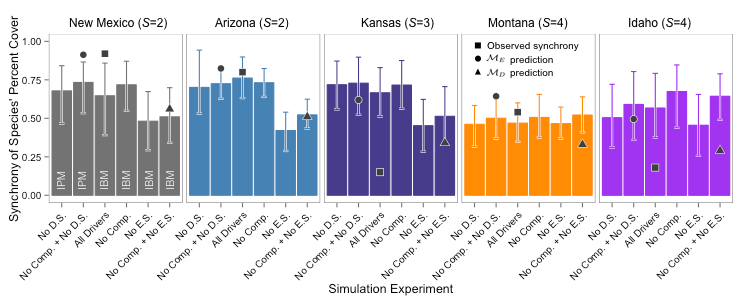
\includegraphics[width=6in]{./components/formatted_figures/formatted_figureS2.png}
  \caption{Community-wide synchrony of species percent cover from model simulation experiments. Synchrony of species' percent cover for each study area are from simulation experiments with demographic stochasticity, environmental stochasticity, and interspecific competition present (``All Drivers''), demographic stochasticity removed (``No D.S.''), environmental stochasticity removed (``No E.S.''), interspecific competition removed (``No Comp.''), interspecific competition and demographic stochasticity removed (``No Comp. + No D.S.''), and interspecific competition and environmental stochasticity removed (``No Comp. + No E.S.''). Abbreviations within the bars for the New Mexico site indicate whether the IBM or IPM was used for a particular simulation. Error bars represent the upper and lower 95\% quantiles from model simulations.}
\end{figure}

\pagebreak{}

\begin{figure}[!ht]
  \centering
      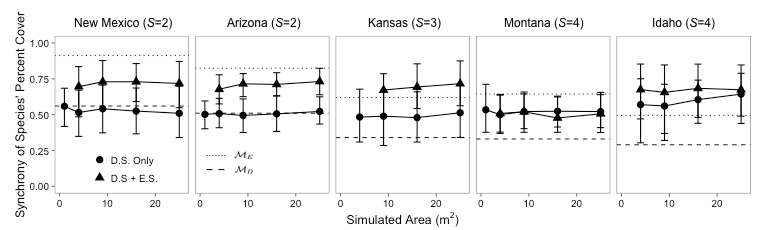
\includegraphics[width=6in]{./components/formatted_figures/formatted_figureS3.png}
  \caption{Synchrony of species' percent cover for each study area from IBM simulations across different landscape sizes when only demographic stochastcity is present (``D.S. Only'') and when environmental stochasticity is also present removed (``D.S. + E.S.''). The strength of demographic stochasticity decreases as landscape size increases because population sizes also increase. Error bars represent the upper and lower 95\% quantiles from model simulations.}
\end{figure}

\pagebreak{}

\begin{figure}[!ht]
  \centering
      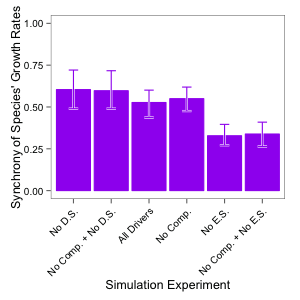
\includegraphics[width=3in]{./components/formatted_figures/formatted_figureS4.png}
  \caption{Community-wide synchrony of species' growth rates from model simulation experiments for the Idaho community with \textit{Artemisia tripartita} removed. Synchrony of species' growth rates are from simulation experiments with demographic stochasticity, environmental stochasticity, and interspecific competition present (``All Drivers''), demographic stochasticity removed (``No D.S.''), environmental stochasticity removed (``No E.S.''), interspecific competition removed (``No Comp.''), interspecific competition and demographic stochasticity removed (``No Comp. + No D.S.''), and interspecific competition and environmental stochasticity removed (``No Comp. + No E.S.''). Error bars represent the upper and lower 95\% quantiles from model simulations.}
\end{figure}

\newpage{}

\subsection{Supporting Tables}\label{supporting-tables}

\begin{table}[ht]
\centering
\caption{Comparisons between our analytical predictions and simulation results for synchrony of species' per capita growth rates. Analytical predictions represent two limiting cases where only demographic stochasticity is operating ($\phi_{R,\mathcal{M}_D}$) and where only environmental stochasticity is operating ($\phi_{R,\mathcal{M}_E}$). Simulated synchrony values come from our empirically-based, multi-species population models when simulated under conditions that match the limiting case conditions (e.g., environmental stochasticity and competition removed for $\mathcal{M}_D$).} 
{\normalsize
\begin{tabular}{lrrrr}
  \hline
Site & Predicted $\phi_{R,\mathcal{M}_D}$ & Simulated $\phi_{R,\mathcal{M}_D}$ & Predicted $\phi_{R,\mathcal{M}_E}$ & Simulated $\phi_{R,\mathcal{M}_E}$ \\ 
  \hline
New Mexico & 0.56 & 0.51 & 0.86 & 0.86 \\ 
  Arizona & 0.51 & 0.52 & 0.82 & 0.82 \\ 
  Kansas & 0.35 & 0.39 & 0.62 & 0.62 \\ 
  Montana & 0.31 & 0.33 & 0.47 & 0.49 \\ 
  Idaho & 0.29 & 0.31 & 0.43 & 0.41 \\ 
   \hline
\end{tabular}
}
\end{table}

\begin{table}[ht]
\centering
\caption{Percent differences of synchrony of per capita growth rates between each removal simulation experiment and the 'All Drivers' simulation.} 
\begin{tabular}{lrrrrr}
  \hline
simulation & 1New Mexico & 2Arizona & 3Kansas & 4Montana & 5Idaho \\ 
  \hline
1No D.S. & 4.82 & 3.99 & 7.19 & 5.37 & 9.53 \\ 
  2No Comp. + No D.S. & 4.74 & 2.70 & 6.81 & 4.53 & 7.69 \\ 
  4No Comp. & 0.98 & 0.06 & 4.84 & 1.01 & 0.11 \\ 
  5No E.S. & 40.14 & 33.20 & 47.84 & 38.52 & 9.28 \\ 
  6No Comp. + No E.S. & 45.95 & 41.48 & 38.21 & 33.07 & 20.33 \\ 
   \hline
\end{tabular}
\end{table}

\begin{table}[ht]
\centering
\caption{Correlations of species' year random effects for each site by term, where term refers to the random effect on the slope or the intercept.} 
\begin{tabular}{llrrr}
  \hline
site & term & growth & recruit & surv \\ 
  \hline
Arizona & intercept & 0.49 & -0.05 & 0.45 \\ 
  Arizona & slope & 0.68 &  & 0.15 \\ 
  Idaho & intercept & 0.46 & 0.38 & 0.29 \\ 
  Idaho & slope & 0.50 &  & 0.47 \\ 
  Kansas & intercept & 0.47 & 0.29 & 0.24 \\ 
  Kansas & slope & 0.18 &  & 0.16 \\ 
  Montana & intercept & 0.26 & 0.04 & 0.39 \\ 
  Montana & slope & 0.10 &  & 0.01 \\ 
  NewMexico & intercept & 0.54 & -0.15 & 0.64 \\ 
  NewMexico & slope & 0.32 &  & 0.15 \\ 
   \hline
\end{tabular}
\end{table}

\begin{table}[ht]
\centering
\caption{Average interaction coefficients for each vital rate for each community.} 
\begin{tabular}{llrrr}
  \hline
Site & Interaction Type & Growth & Recruitment & Survival \\ 
  \hline
Arizona & Interspecific & -0.0111 & -0.4534 & -0.0507 \\ 
  Arizona & Intraspecific & -0.0402 & -1.4209 & -0.4446 \\ 
  Idaho & Interspecific & 0.0022 & -0.1091 & 0.0059 \\ 
  Idaho & Intraspecific & -0.0469 & -1.5569 & -0.5269 \\ 
  Kansas & Interspecific & -0.0008 & 0.0463 & -0.0041 \\ 
  Kansas & Intraspecific & -0.0062 & -0.9945 & -0.0586 \\ 
  Montana & Interspecific & -0.0053 & 0.0920 & 0.0354 \\ 
  Montana & Intraspecific & -0.0733 & -2.0492 & -0.8103 \\ 
  NewMexico & Interspecific & -0.0027 & -0.3461 & -0.0080 \\ 
  NewMexico & Intraspecific & -0.0111 & -1.6473 & -0.2191 \\ 
   \hline
\end{tabular}
\end{table}

\begin{table}[ht]
\centering
\caption{Interaction coefficients for growth regressions in Arizona.} 
\begin{tabular}{rrr}
  \hline
 & BOER & BORO \\ 
  \hline
BOER & -0.0033 & -0.0171 \\ 
  BORO & -0.0050 & -0.0772 \\ 
   \hline
\end{tabular}
\end{table}\begin{table}[ht]
\centering
\caption{Interaction coefficients for growth regressions in Idaho.} 
\begin{tabular}{rrrrr}
  \hline
 & ARTR & HECO & POSE & PSSP \\ 
  \hline
ARTR & -0.0300 & 0.0129 & 0.0117 & 0.0003 \\ 
  HECO & -0.0000 & -0.0285 & 0.0084 & -0.0028 \\ 
  POSE & 0.0001 & 0.0032 & -0.0845 & -0.0043 \\ 
  PSSP & -0.0003 & -0.0027 & -0.0004 & -0.0448 \\ 
   \hline
\end{tabular}
\end{table}\begin{table}[ht]
\centering
\caption{Interaction coefficients for growth regressions in Kansas.} 
\begin{tabular}{rrrr}
  \hline
 & BOCU & BOHI & SCSC \\ 
  \hline
BOCU & -0.0017 & 0.0011 & 0.0010 \\ 
  BOHI & 0.0002 & -0.0046 & -0.0078 \\ 
  SCSC & -0.0003 & 0.0007 & -0.0124 \\ 
   \hline
\end{tabular}
\end{table}\begin{table}[ht]
\centering
\caption{Interaction coefficients for growth regressions in Montana.} 
\begin{tabular}{rrrrr}
  \hline
 & BOGR & HECO & PASM & POSE \\ 
  \hline
BOGR & -0.0121 & -0.0002 & -0.0229 & -0.0014 \\ 
  HECO & -0.0023 & -0.0778 & 0.0142 & 0.0061 \\ 
  PASM & -0.0005 & -0.0039 & -0.0601 & -0.0033 \\ 
  POSE & 0.0005 & -0.0101 & -0.0404 & -0.1431 \\ 
   \hline
\end{tabular}
\end{table}\begin{table}[ht]
\centering
\caption{Interaction coefficients for growth regressions in NewMexico.} 
\begin{tabular}{rrr}
  \hline
 & BOER & SPFL \\ 
  \hline
BOER & -0.0045 & -0.0013 \\ 
  SPFL & -0.0041 & -0.0176 \\ 
   \hline
\end{tabular}
\end{table}\begin{table}[ht]
\centering
\caption{Interaction coefficients for survival regressions in Arizona.} 
\begin{tabular}{rrr}
  \hline
 & BOER & BORO \\ 
  \hline
BOER & -0.2791 & -0.0816 \\ 
  BORO & -0.0200 & -0.6101 \\ 
   \hline
\end{tabular}
\end{table}\begin{table}[ht]
\centering
\caption{Interaction coefficients for survival regressions in Idaho.} 
\begin{tabular}{rrrrr}
  \hline
 & ARTR & HECO & POSE & PSSP \\ 
  \hline
ARTR & -0.0236 & -0.0202 & 0.0314 & 0.0158 \\ 
  HECO & -0.0005 & -1.0206 & -0.0052 & 0.0125 \\ 
  POSE & 0.0001 & 0.0006 & -0.9091 & 0.0121 \\ 
  PSSP & 0.0009 & -0.0013 & 0.0246 & -0.1543 \\ 
   \hline
\end{tabular}
\end{table}\begin{table}[ht]
\centering
\caption{Interaction coefficients for survival regressions in Kansas.} 
\begin{tabular}{rrrr}
  \hline
 & BOCU & BOHI & SCSC \\ 
  \hline
BOCU & -0.1087 & 0.0006 & 0.0010 \\ 
  BOHI & 0.0021 & -0.0403 & -0.0153 \\ 
  SCSC & -0.0064 & -0.0066 & -0.0270 \\ 
   \hline
\end{tabular}
\end{table}\begin{table}[ht]
\centering
\caption{Interaction coefficients for survival regressions in Montana.} 
\begin{tabular}{rrrrr}
  \hline
 & BOGR & HECO & PASM & POSE \\ 
  \hline
BOGR & -0.1280 & 0.0211 & 0.1243 & 0.0173 \\ 
  HECO & -0.0043 & -0.5661 & 0.1386 & 0.0013 \\ 
  PASM & 0.0001 & -0.0044 & -1.3046 & 0.0012 \\ 
  POSE & 0.0010 & 0.0085 & 0.1198 & -1.2434 \\ 
   \hline
\end{tabular}
\end{table}\begin{table}[ht]
\centering
\caption{Interaction coefficients for survival regressions in NewMexico.} 
\begin{tabular}{rrr}
  \hline
 & BOER & SPFL \\ 
  \hline
BOER & -0.1575 & -0.0040 \\ 
  SPFL & -0.0120 & -0.2807 \\ 
   \hline
\end{tabular}
\end{table}\begin{table}[ht]
\centering
\caption{Interaction coefficients for recruitment regressions in Arizona.} 
\begin{tabular}{rrr}
  \hline
 & BOER & BORO \\ 
  \hline
BOER & -0.5304 & -0.3063 \\ 
  BORO & -0.5798 & -2.3237 \\ 
   \hline
\end{tabular}
\end{table}\begin{table}[ht]
\centering
\caption{Interaction coefficients for recruitment regressions in Idaho.} 
\begin{tabular}{rrrrr}
  \hline
 & ARTR & HECO & POSE & PSSP \\ 
  \hline
ARTR & -0.4054 & 0.2132 & 0.0120 & 0.2389 \\ 
  HECO & -0.5674 & -1.7722 & -0.1476 & -0.3184 \\ 
  POSE & -0.2499 & -0.0328 & -2.2873 & -0.1448 \\ 
  PSSP & -0.2580 & -0.1687 & 0.0365 & -1.7675 \\ 
   \hline
\end{tabular}
\end{table}\begin{table}[ht]
\centering
\caption{Interaction coefficients for recruitment regressions in Kansas.} 
\begin{tabular}{rrrr}
  \hline
 & BOCU & BOHI & SCSC \\ 
  \hline
BOCU & -1.1584 & -0.0242 & -0.0524 \\ 
  BOHI & 0.3387 & -0.8620 & 0.0123 \\ 
  SCSC & 0.0615 & -0.0308 & -0.9543 \\ 
   \hline
\end{tabular}
\end{table}\begin{table}[ht]
\centering
\caption{Interaction coefficients for recruitment regressions in Montana.} 
\begin{tabular}{rrrrr}
  \hline
 & BOGR & HECO & PASM & POSE \\ 
  \hline
BOGR & -0.8916 & -0.2522 & -0.1334 & 0.0610 \\ 
  HECO & 0.0852 & -1.4191 & -0.0685 & -0.0422 \\ 
  PASM & 0.1252 & 0.3093 & -4.1823 & 0.3032 \\ 
  POSE & 0.1577 & 0.4906 & 0.0709 & -1.7065 \\ 
   \hline
\end{tabular}
\end{table}\begin{table}[ht]
\centering
\caption{Interaction coefficients for recruitment regressions in NewMexico.} 
\begin{tabular}{rrr}
  \hline
 & BOER & SPFL \\ 
  \hline
BOER & -0.7631 & -0.6198 \\ 
  SPFL & -0.0684 & -2.5220 \\ 
   \hline
\end{tabular}
\end{table}

\newpage{}

\begin{table}[ht]
\centering
\caption{Parameter correlations for site = Arizona, vital rate = growth, and species = BOER.} 
\begin{tabular}{rrrrr}
  \hline
 & (Intercept) & logarea.t0 & crowdV1 & crowdV2 \\ 
  \hline
(Intercept) & 1.00E+00 & -1.34E-01 & -1.15E-01 & -9.09E-02 \\ 
  logarea.t0 & -1.34E-01 & 1.00E+00 & -2.09E-02 & 3.67E-02 \\ 
  crowdV1 & -1.15E-01 & -2.09E-02 & 1.00E+00 & 1.02E-01 \\ 
  crowdV2 & -9.09E-02 & 3.67E-02 & 1.02E-01 & 1.00E+00 \\ 
   \hline
\end{tabular}
\end{table}

\begin{table}[ht]
\centering
\caption{Parameter correlations for site = Arizona, vital rate = growth, and species = BORO.} 
\begin{tabular}{rrrrr}
  \hline
 & (Intercept) & logarea.t0 & crowdV1 & crowdV2 \\ 
  \hline
(Intercept) & 1.00E+00 & -5.64E-02 & -7.69E-02 & -7.72E-02 \\ 
  logarea.t0 & -5.64E-02 & 1.00E+00 & 3.00E-02 & 3.60E-04 \\ 
  crowdV1 & -7.69E-02 & 3.00E-02 & 1.00E+00 & 6.23E-02 \\ 
  crowdV2 & -7.72E-02 & 3.60E-04 & 6.23E-02 & 1.00E+00 \\ 
   \hline
\end{tabular}
\end{table}

\begin{table}[ht]
\centering
\caption{Parameter correlations for site = Idaho, vital rate = growth, and species = ARTR.} 
\begin{tabular}{rrrrrrr}
  \hline
 & (Intercept) & logarea.t0 & crowdV1 & crowdV2 & crowdV3 & crowdV4 \\ 
  \hline
(Intercept) & 1.00E+00 & -8.98E-02 & -4.69E-02 & -4.01E-02 & -2.91E-02 & -7.15E-02 \\ 
  logarea.t0 & -8.98E-02 & 1.00E+00 & 3.69E-02 & 5.78E-03 & 5.03E-05 & -3.27E-03 \\ 
  crowdV1 & -4.69E-02 & 3.69E-02 & 1.00E+00 & -1.67E-02 & -3.06E-02 & -1.05E-03 \\ 
  crowdV2 & -4.01E-02 & 5.78E-03 & -1.67E-02 & 1.00E+00 & -2.54E-02 & 8.19E-02 \\ 
  crowdV3 & -2.91E-02 & 5.03E-05 & -3.06E-02 & -2.54E-02 & 1.00E+00 & 3.12E-02 \\ 
  crowdV4 & -7.15E-02 & -3.27E-03 & -1.05E-03 & 8.19E-02 & 3.12E-02 & 1.00E+00 \\ 
   \hline
\end{tabular}
\end{table}

\newpage{}

\begin{table}[ht]
\centering
\caption{Parameter correlations for site = Idaho, vital rate = growth, and species = HECO.} 
\begin{tabular}{rrrrrrr}
  \hline
 & (Intercept) & logarea.t0 & crowdV1 & crowdV2 & crowdV3 & crowdV4 \\ 
  \hline
(Intercept) & 1.00E+00 & -1.25E-01 & -4.30E-02 & -1.10E-01 & -6.36E-02 & -1.03E-01 \\ 
  logarea.t0 & -1.25E-01 & 1.00E+00 & 4.95E-03 & 5.15E-02 & 2.80E-03 & 6.47E-02 \\ 
  crowdV1 & -4.30E-02 & 4.95E-03 & 1.00E+00 & -1.11E-02 & 2.73E-02 & 6.86E-02 \\ 
  crowdV2 & -1.10E-01 & 5.15E-02 & -1.11E-02 & 1.00E+00 & -5.17E-02 & 5.57E-02 \\ 
  crowdV3 & -6.36E-02 & 2.80E-03 & 2.73E-02 & -5.17E-02 & 1.00E+00 & 1.17E-02 \\ 
  crowdV4 & -1.03E-01 & 6.47E-02 & 6.86E-02 & 5.57E-02 & 1.17E-02 & 1.00E+00 \\ 
   \hline
\end{tabular}
\end{table}

\begin{table}[ht]
\centering
\caption{Parameter correlations for site = Idaho, vital rate = growth, and species = POSE.} 
\begin{tabular}{rrrrrrr}
  \hline
 & (Intercept) & logarea.t0 & crowdV1 & crowdV2 & crowdV3 & crowdV4 \\ 
  \hline
(Intercept) & 1.00E+00 & -9.56E-02 & -4.68E-02 & -8.67E-02 & -7.52E-02 & -1.32E-01 \\ 
  logarea.t0 & -9.56E-02 & 1.00E+00 & 1.29E-02 & 1.77E-03 & 9.43E-03 & 4.44E-02 \\ 
  crowdV1 & -4.68E-02 & 1.29E-02 & 1.00E+00 & 4.50E-02 & 7.39E-03 & 5.64E-02 \\ 
  crowdV2 & -8.67E-02 & 1.77E-03 & 4.50E-02 & 1.00E+00 & -5.26E-03 & 7.84E-02 \\ 
  crowdV3 & -7.52E-02 & 9.43E-03 & 7.39E-03 & -5.26E-03 & 1.00E+00 & 1.48E-02 \\ 
  crowdV4 & -1.32E-01 & 4.44E-02 & 5.64E-02 & 7.84E-02 & 1.48E-02 & 1.00E+00 \\ 
   \hline
\end{tabular}
\end{table}

\begin{table}[ht]
\centering
\caption{Parameter correlations for site = Idaho, vital rate = growth, and species = PSSP.} 
\begin{tabular}{rrrrrrr}
  \hline
 & (Intercept) & logarea.t0 & crowdV1 & crowdV2 & crowdV3 & crowdV4 \\ 
  \hline
(Intercept) & 1.00E+00 & -8.15E-02 & -4.77E-02 & -5.04E-02 & -6.31E-02 & -8.25E-02 \\ 
  logarea.t0 & -8.15E-02 & 1.00E+00 & 3.28E-02 & 3.53E-02 & 1.95E-02 & 3.99E-02 \\ 
  crowdV1 & -4.77E-02 & 3.28E-02 & 1.00E+00 & 3.60E-02 & 1.27E-02 & -9.47E-03 \\ 
  crowdV2 & -5.04E-02 & 3.53E-02 & 3.60E-02 & 1.00E+00 & -1.01E-02 & 1.52E-02 \\ 
  crowdV3 & -6.31E-02 & 1.95E-02 & 1.27E-02 & -1.01E-02 & 1.00E+00 & 2.27E-02 \\ 
  crowdV4 & -8.25E-02 & 3.99E-02 & -9.47E-03 & 1.52E-02 & 2.27E-02 & 1.00E+00 \\ 
   \hline
\end{tabular}
\end{table}

\newpage{}

\begin{table}[ht]
\centering
\caption{Parameter correlations for site = Kansas, vital rate = growth, and species = BOCU.} 
\begin{tabular}{rrrrrr}
  \hline
 & (Intercept) & logarea.t0 & crowdV1 & crowdV2 & crowdV3 \\ 
  \hline
(Intercept) & 1.00E+00 & -1.27E-01 & -7.88E-02 & -6.53E-02 & -2.72E-02 \\ 
  logarea.t0 & -1.27E-01 & 1.00E+00 & 7.37E-02 & 8.64E-02 & 4.48E-02 \\ 
  crowdV1 & -7.88E-02 & 7.37E-02 & 1.00E+00 & -1.12E-02 & 2.39E-02 \\ 
  crowdV2 & -6.53E-02 & 8.64E-02 & -1.12E-02 & 1.00E+00 & 6.34E-02 \\ 
  crowdV3 & -2.72E-02 & 4.48E-02 & 2.39E-02 & 6.34E-02 & 1.00E+00 \\ 
   \hline
\end{tabular}
\end{table}

\begin{table}[ht]
\centering
\caption{Parameter correlations for site = Kansas, vital rate = growth, and species = BOHI.} 
\begin{tabular}{rrrrrr}
  \hline
 & (Intercept) & logarea.t0 & crowdV1 & crowdV2 & crowdV3 \\ 
  \hline
(Intercept) & 1.00E+00 & -1.27E-01 & -3.75E-02 & -3.16E-02 & -3.57E-02 \\ 
  logarea.t0 & -1.27E-01 & 1.00E+00 & 5.16E-02 & 7.55E-02 & 1.74E-01 \\ 
  crowdV1 & -3.75E-02 & 5.16E-02 & 1.00E+00 & -6.11E-02 & 3.83E-02 \\ 
  crowdV2 & -3.16E-02 & 7.55E-02 & -6.11E-02 & 1.00E+00 & 6.58E-02 \\ 
  crowdV3 & -3.57E-02 & 1.74E-01 & 3.83E-02 & 6.58E-02 & 1.00E+00 \\ 
   \hline
\end{tabular}
\end{table}

\begin{table}[ht]
\centering
\caption{Parameter correlations for site = Kansas, vital rate = growth, and species = SCSC.} 
\begin{tabular}{rrrrrr}
  \hline
 & (Intercept) & logarea.t0 & crowdV1 & crowdV2 & crowdV3 \\ 
  \hline
(Intercept) & 1.00E+00 & -2.59E-01 & -1.43E-01 & -7.78E-02 & -9.80E-02 \\ 
  logarea.t0 & -2.59E-01 & 1.00E+00 & 2.02E-01 & 1.85E-01 & 2.40E-01 \\ 
  crowdV1 & -1.43E-01 & 2.02E-01 & 1.00E+00 & 4.84E-02 & 9.45E-02 \\ 
  crowdV2 & -7.78E-02 & 1.85E-01 & 4.84E-02 & 1.00E+00 & 2.75E-02 \\ 
  crowdV3 & -9.80E-02 & 2.40E-01 & 9.45E-02 & 2.75E-02 & 1.00E+00 \\ 
   \hline
\end{tabular}
\end{table}

\newpage{}

\begin{table}[ht]
\centering
\caption{Parameter correlations for site = Montana, vital rate = growth, and species = BOGR.} 
\begin{tabular}{rrrrrrr}
  \hline
 & (Intercept) & logarea.t0 & crowdV1 & crowdV2 & crowdV3 & crowdV4 \\ 
  \hline
(Intercept) & 1.00E+00 & -4.52E-02 & -7.52E-02 & -3.67E-02 & -4.32E-02 & -2.79E-02 \\ 
  logarea.t0 & -4.52E-02 & 1.00E+00 & 2.29E-02 & 1.73E-02 & 1.72E-02 & 2.35E-03 \\ 
  crowdV1 & -7.52E-02 & 2.29E-02 & 1.00E+00 & 3.98E-02 & -6.01E-02 & -6.43E-03 \\ 
  crowdV2 & -3.67E-02 & 1.73E-02 & 3.98E-02 & 1.00E+00 & 3.07E-02 & 2.20E-02 \\ 
  crowdV3 & -4.32E-02 & 1.72E-02 & -6.01E-02 & 3.07E-02 & 1.00E+00 & 2.40E-02 \\ 
  crowdV4 & -2.79E-02 & 2.35E-03 & -6.43E-03 & 2.20E-02 & 2.40E-02 & 1.00E+00 \\ 
   \hline
\end{tabular}
\end{table}

\begin{table}[ht]
\centering
\caption{Parameter correlations for site = Montana, vital rate = growth, and species = HECO.} 
\begin{tabular}{rrrrrrr}
  \hline
 & (Intercept) & logarea.t0 & crowdV1 & crowdV2 & crowdV3 & crowdV4 \\ 
  \hline
(Intercept) & 1.00E+00 & -2.31E-02 & -8.93E-02 & -5.50E-02 & -9.75E-02 & -4.23E-02 \\ 
  logarea.t0 & -2.31E-02 & 1.00E+00 & 1.75E-02 & -2.02E-02 & 1.17E-03 & 1.38E-02 \\ 
  crowdV1 & -8.93E-02 & 1.75E-02 & 1.00E+00 & 9.21E-02 & 5.16E-02 & -1.44E-02 \\ 
  crowdV2 & -5.50E-02 & -2.02E-02 & 9.21E-02 & 1.00E+00 & 3.90E-02 & -3.61E-03 \\ 
  crowdV3 & -9.75E-02 & 1.17E-03 & 5.16E-02 & 3.90E-02 & 1.00E+00 & 3.92E-02 \\ 
  crowdV4 & -4.23E-02 & 1.38E-02 & -1.44E-02 & -3.61E-03 & 3.92E-02 & 1.00E+00 \\ 
   \hline
\end{tabular}
\end{table}

\begin{table}[ht]
\centering
\caption{Parameter correlations for site = Montana, vital rate = growth, and species = PASM.} 
\begin{tabular}{rrrrrrr}
  \hline
 & (Intercept) & logarea.t0 & crowdV1 & crowdV2 & crowdV3 & crowdV4 \\ 
  \hline
(Intercept) & 1.00E+00 & 1.65E-02 & -6.08E-02 & -4.11E-02 & -1.10E-01 & -2.98E-02 \\ 
  logarea.t0 & 1.65E-02 & 1.00E+00 & 4.15E-03 & 4.42E-03 & -7.75E-03 & 1.04E-02 \\ 
  crowdV1 & -6.08E-02 & 4.15E-03 & 1.00E+00 & 9.00E-02 & 8.59E-02 & -3.36E-02 \\ 
  crowdV2 & -4.11E-02 & 4.42E-03 & 9.00E-02 & 1.00E+00 & 2.85E-02 & 1.31E-02 \\ 
  crowdV3 & -1.10E-01 & -7.75E-03 & 8.59E-02 & 2.85E-02 & 1.00E+00 & 3.59E-03 \\ 
  crowdV4 & -2.98E-02 & 1.04E-02 & -3.36E-02 & 1.31E-02 & 3.59E-03 & 1.00E+00 \\ 
   \hline
\end{tabular}
\end{table}

\newpage{}

\begin{table}[ht]
\centering
\caption{Parameter correlations for site = Montana, vital rate = growth, and species = POSE.} 
\begin{tabular}{rrrrrrr}
  \hline
 & (Intercept) & logarea.t0 & crowdV1 & crowdV2 & crowdV3 & crowdV4 \\ 
  \hline
(Intercept) & 1.00E+00 & -4.09E-02 & -6.28E-02 & -3.56E-02 & -8.91E-02 & -4.55E-02 \\ 
  logarea.t0 & -4.09E-02 & 1.00E+00 & -8.02E-03 & 2.17E-02 & 4.47E-02 & 1.00E-02 \\ 
  crowdV1 & -6.28E-02 & -8.02E-03 & 1.00E+00 & 1.03E-01 & 6.54E-02 & 9.60E-03 \\ 
  crowdV2 & -3.56E-02 & 2.17E-02 & 1.03E-01 & 1.00E+00 & 5.30E-02 & 4.18E-02 \\ 
  crowdV3 & -8.91E-02 & 4.47E-02 & 6.54E-02 & 5.30E-02 & 1.00E+00 & 2.95E-02 \\ 
  crowdV4 & -4.55E-02 & 1.00E-02 & 9.60E-03 & 4.18E-02 & 2.95E-02 & 1.00E+00 \\ 
   \hline
\end{tabular}
\end{table}

\begin{table}[ht]
\centering
\caption{Parameter correlations for site = NewMexico, vital rate = growth, and species = BOER.} 
\begin{tabular}{rrrrr}
  \hline
 & (Intercept) & logarea.t0 & crowdV1 & crowdV2 \\ 
  \hline
(Intercept) & 1.00E+00 & -1.33E-01 & -1.25E-01 & -3.79E-02 \\ 
  logarea.t0 & -1.33E-01 & 1.00E+00 & 3.30E-02 & 2.14E-02 \\ 
  crowdV1 & -1.25E-01 & 3.30E-02 & 1.00E+00 & 5.46E-02 \\ 
  crowdV2 & -3.79E-02 & 2.14E-02 & 5.46E-02 & 1.00E+00 \\ 
   \hline
\end{tabular}
\end{table}

\begin{table}[ht]
\centering
\caption{Parameter correlations for site = NewMexico, vital rate = growth, and species = SPFL.} 
\begin{tabular}{rrrrr}
  \hline
 & (Intercept) & logarea.t0 & crowdV1 & crowdV2 \\ 
  \hline
(Intercept) & 1.00E+00 & -3.24E-01 & -1.29E-01 & -9.84E-02 \\ 
  logarea.t0 & -3.24E-01 & 1.00E+00 & 3.89E-02 & 4.28E-02 \\ 
  crowdV1 & -1.29E-01 & 3.89E-02 & 1.00E+00 & 3.82E-02 \\ 
  crowdV2 & -9.84E-02 & 4.28E-02 & 3.82E-02 & 1.00E+00 \\ 
   \hline
\end{tabular}
\end{table}

\newpage{}

\begin{table}[ht]
\centering
\caption{Parameter correlations for site = Arizona, vital rate = surv, and species = BOER.} 
\begin{tabular}{rrrrr}
  \hline
 & (Intercept) & logarea & crowdV1 & crowdV2 \\ 
  \hline
(Intercept) & 1.00E+00 & -1.36E-01 & -9.25E-02 & -9.08E-02 \\ 
  logarea & -1.36E-01 & 1.00E+00 & -3.15E-02 & 1.56E-02 \\ 
  crowdV1 & -9.25E-02 & -3.15E-02 & 1.00E+00 & 3.54E-02 \\ 
  crowdV2 & -9.08E-02 & 1.56E-02 & 3.54E-02 & 1.00E+00 \\ 
   \hline
\end{tabular}
\end{table}

\begin{table}[ht]
\centering
\caption{Parameter correlations for site = Arizona, vital rate = surv, and species = BORO.} 
\begin{tabular}{rrrrr}
  \hline
 & (Intercept) & logarea & crowdV1 & crowdV2 \\ 
  \hline
(Intercept) & 1.00E+00 & -8.81E-03 & -2.77E-02 & -5.40E-02 \\ 
  logarea & -8.81E-03 & 1.00E+00 & 1.02E-02 & -1.25E-02 \\ 
  crowdV1 & -2.77E-02 & 1.02E-02 & 1.00E+00 & 5.37E-02 \\ 
  crowdV2 & -5.40E-02 & -1.25E-02 & 5.37E-02 & 1.00E+00 \\ 
   \hline
\end{tabular}
\end{table}

\begin{table}[ht]
\centering
\caption{Parameter correlations for site = Idaho, vital rate = surv, and species = ARTR.} 
\begin{tabular}{rrrrrrr}
  \hline
 & (Intercept) & logarea & crowdV1 & crowdV2 & crowdV3 & crowdV4 \\ 
  \hline
(Intercept) & 1.00E+00 & -1.73E-01 & -2.05E-01 & -6.82E-02 & -7.73E-02 & -2.43E-01 \\ 
  logarea & -1.73E-01 & 1.00E+00 & 1.66E-04 & -2.14E-02 & 1.31E-02 & 6.83E-02 \\ 
  crowdV1 & -2.05E-01 & 1.66E-04 & 1.00E+00 & -2.11E-02 & -2.09E-02 & 2.15E-02 \\ 
  crowdV2 & -6.82E-02 & -2.14E-02 & -2.11E-02 & 1.00E+00 & -3.73E-04 & 3.67E-02 \\ 
  crowdV3 & -7.73E-02 & 1.31E-02 & -2.09E-02 & -3.73E-04 & 1.00E+00 & 1.82E-02 \\ 
  crowdV4 & -2.43E-01 & 6.83E-02 & 2.15E-02 & 3.67E-02 & 1.82E-02 & 1.00E+00 \\ 
   \hline
\end{tabular}
\end{table}

\newpage{}

\begin{table}[ht]
\centering
\caption{Parameter correlations for site = Idaho, vital rate = surv, and species = HECO.} 
\begin{tabular}{rrrrrrr}
  \hline
 & (Intercept) & logarea & crowdV1 & crowdV2 & crowdV3 & crowdV4 \\ 
  \hline
(Intercept) & 1.00E+00 & 6.74E-02 & -8.51E-02 & -1.31E-01 & -8.00E-02 & -1.08E-01 \\ 
  logarea & 6.74E-02 & 1.00E+00 & 1.65E-02 & -2.28E-02 & -1.04E-02 & 1.87E-02 \\ 
  crowdV1 & -8.51E-02 & 1.65E-02 & 1.00E+00 & -8.42E-03 & 1.36E-02 & 1.27E-01 \\ 
  crowdV2 & -1.31E-01 & -2.28E-02 & -8.42E-03 & 1.00E+00 & 2.71E-03 & 3.61E-02 \\ 
  crowdV3 & -8.00E-02 & -1.04E-02 & 1.36E-02 & 2.71E-03 & 1.00E+00 & -8.60E-03 \\ 
  crowdV4 & -1.08E-01 & 1.87E-02 & 1.27E-01 & 3.61E-02 & -8.60E-03 & 1.00E+00 \\ 
   \hline
\end{tabular}
\end{table}

\begin{table}[ht]
\centering
\caption{Parameter correlations for site = Idaho, vital rate = surv, and species = POSE.} 
\begin{tabular}{rrrrrrr}
  \hline
 & (Intercept) & logarea & crowdV1 & crowdV2 & crowdV3 & crowdV4 \\ 
  \hline
(Intercept) & 1.00E+00 & 5.11E-02 & -6.64E-02 & -5.27E-02 & -7.80E-02 & -1.01E-01 \\ 
  logarea & 5.11E-02 & 1.00E+00 & 1.46E-02 & 6.55E-03 & -2.42E-02 & 1.35E-03 \\ 
  crowdV1 & -6.64E-02 & 1.46E-02 & 1.00E+00 & 6.15E-02 & -2.11E-02 & 6.79E-02 \\ 
  crowdV2 & -5.27E-02 & 6.55E-03 & 6.15E-02 & 1.00E+00 & 5.89E-03 & 6.17E-02 \\ 
  crowdV3 & -7.80E-02 & -2.42E-02 & -2.11E-02 & 5.89E-03 & 1.00E+00 & -1.04E-01 \\ 
  crowdV4 & -1.01E-01 & 1.35E-03 & 6.79E-02 & 6.17E-02 & -1.04E-01 & 1.00E+00 \\ 
   \hline
\end{tabular}
\end{table}

\begin{table}[ht]
\centering
\caption{Parameter correlations for site = Idaho, vital rate = surv, and species = PSSP.} 
\begin{tabular}{rrrrrrr}
  \hline
 & (Intercept) & logarea & crowdV1 & crowdV2 & crowdV3 & crowdV4 \\ 
  \hline
(Intercept) & 1.00E+00 & 6.03E-02 & -6.59E-02 & -2.53E-02 & -5.16E-02 & -9.37E-02 \\ 
  logarea & 6.03E-02 & 1.00E+00 & 1.46E-02 & 7.86E-03 & -3.97E-03 & -4.80E-02 \\ 
  crowdV1 & -6.59E-02 & 1.46E-02 & 1.00E+00 & 1.28E-02 & 1.80E-02 & 3.74E-02 \\ 
  crowdV2 & -2.53E-02 & 7.86E-03 & 1.28E-02 & 1.00E+00 & -4.17E-03 & 2.34E-02 \\ 
  crowdV3 & -5.16E-02 & -3.97E-03 & 1.80E-02 & -4.17E-03 & 1.00E+00 & 2.05E-02 \\ 
  crowdV4 & -9.37E-02 & -4.80E-02 & 3.74E-02 & 2.34E-02 & 2.05E-02 & 1.00E+00 \\ 
   \hline
\end{tabular}
\end{table}

\newpage{}

\begin{table}[ht]
\centering
\caption{Parameter correlations for site = Kansas, vital rate = surv, and species = BOCU.} 
\begin{tabular}{rrrrrr}
  \hline
 & (Intercept) & logarea & crowdV1 & crowdV2 & crowdV3 \\ 
  \hline
(Intercept) & 1.00E+00 & -2.04E-01 & -5.64E-02 & -7.87E-02 & -5.55E-02 \\ 
  logarea & -2.04E-01 & 1.00E+00 & -2.86E-02 & 3.25E-02 & 1.81E-02 \\ 
  crowdV1 & -5.64E-02 & -2.86E-02 & 1.00E+00 & -3.70E-02 & 4.25E-02 \\ 
  crowdV2 & -7.87E-02 & 3.25E-02 & -3.70E-02 & 1.00E+00 & 1.10E-01 \\ 
  crowdV3 & -5.55E-02 & 1.81E-02 & 4.25E-02 & 1.10E-01 & 1.00E+00 \\ 
   \hline
\end{tabular}
\end{table}

\begin{table}[ht]
\centering
\caption{Parameter correlations for site = Kansas, vital rate = surv, and species = BOHI.} 
\begin{tabular}{rrrrrr}
  \hline
 & (Intercept) & logarea & crowdV1 & crowdV2 & crowdV3 \\ 
  \hline
(Intercept) & 1.00E+00 & -1.09E-01 & -2.29E-02 & -2.75E-02 & -1.80E-02 \\ 
  logarea & -1.09E-01 & 1.00E+00 & -8.16E-03 & -6.52E-02 & -2.59E-02 \\ 
  crowdV1 & -2.29E-02 & -8.16E-03 & 1.00E+00 & 5.98E-02 & 3.19E-02 \\ 
  crowdV2 & -2.75E-02 & -6.52E-02 & 5.98E-02 & 1.00E+00 & 1.07E-01 \\ 
  crowdV3 & -1.80E-02 & -2.59E-02 & 3.19E-02 & 1.07E-01 & 1.00E+00 \\ 
   \hline
\end{tabular}
\end{table}

\begin{table}[ht]
\centering
\caption{Parameter correlations for site = Kansas, vital rate = surv, and species = SCSC.} 
\begin{tabular}{rrrrrr}
  \hline
 & (Intercept) & logarea & crowdV1 & crowdV2 & crowdV3 \\ 
  \hline
(Intercept) & 1.00E+00 & -1.84E-01 & -3.85E-02 & -3.41E-02 & -4.71E-02 \\ 
  logarea & -1.84E-01 & 1.00E+00 & 1.41E-02 & -1.72E-02 & -6.63E-04 \\ 
  crowdV1 & -3.85E-02 & 1.41E-02 & 1.00E+00 & 5.31E-02 & 5.63E-02 \\ 
  crowdV2 & -3.41E-02 & -1.72E-02 & 5.31E-02 & 1.00E+00 & 7.50E-02 \\ 
  crowdV3 & -4.71E-02 & -6.63E-04 & 5.63E-02 & 7.50E-02 & 1.00E+00 \\ 
   \hline
\end{tabular}
\end{table}

\newpage{}

\begin{table}[ht]
\centering
\caption{Parameter correlations for site = Montana, vital rate = surv, and species = BOGR.} 
\begin{tabular}{rrrrrrr}
  \hline
 & (Intercept) & logarea & crowdV1 & crowdV2 & crowdV3 & crowdV4 \\ 
  \hline
(Intercept) & 1.00E+00 & -2.42E-02 & -6.26E-02 & -3.93E-02 & -4.13E-02 & -3.32E-02 \\ 
  logarea & -2.42E-02 & 1.00E+00 & -1.46E-02 & 1.17E-02 & 1.22E-02 & 4.58E-03 \\ 
  crowdV1 & -6.26E-02 & -1.46E-02 & 1.00E+00 & 2.74E-02 & -6.18E-02 & -2.90E-02 \\ 
  crowdV2 & -3.93E-02 & 1.17E-02 & 2.74E-02 & 1.00E+00 & 1.82E-02 & 2.28E-02 \\ 
  crowdV3 & -4.13E-02 & 1.22E-02 & -6.18E-02 & 1.82E-02 & 1.00E+00 & 2.29E-02 \\ 
  crowdV4 & -3.32E-02 & 4.58E-03 & -2.90E-02 & 2.28E-02 & 2.29E-02 & 1.00E+00 \\ 
   \hline
\end{tabular}
\end{table}

\begin{table}[ht]
\centering
\caption{Parameter correlations for site = Montana, vital rate = surv, and species = HECO.} 
\begin{tabular}{rrrrrrr}
  \hline
 & (Intercept) & logarea & crowdV1 & crowdV2 & crowdV3 & crowdV4 \\ 
  \hline
(Intercept) & 1.00E+00 & 5.49E-02 & -6.27E-02 & -7.44E-02 & -8.86E-02 & -4.69E-02 \\ 
  logarea & 5.49E-02 & 1.00E+00 & -4.33E-03 & -4.33E-02 & 1.92E-02 & 1.60E-02 \\ 
  crowdV1 & -6.27E-02 & -4.33E-03 & 1.00E+00 & 5.86E-02 & 2.63E-02 & -1.98E-02 \\ 
  crowdV2 & -7.44E-02 & -4.33E-02 & 5.86E-02 & 1.00E+00 & 4.25E-02 & 2.18E-02 \\ 
  crowdV3 & -8.86E-02 & 1.92E-02 & 2.63E-02 & 4.25E-02 & 1.00E+00 & 4.26E-02 \\ 
  crowdV4 & -4.69E-02 & 1.60E-02 & -1.98E-02 & 2.18E-02 & 4.26E-02 & 1.00E+00 \\ 
   \hline
\end{tabular}
\end{table}

\begin{table}[ht]
\centering
\caption{Parameter correlations for site = Montana, vital rate = surv, and species = PASM.} 
\begin{tabular}{rrrrrrr}
  \hline
 & (Intercept) & logarea & crowdV1 & crowdV2 & crowdV3 & crowdV4 \\ 
  \hline
(Intercept) & 1.00E+00 & 1.01E-01 & -2.99E-02 & -2.06E-02 & -7.10E-02 & -2.57E-02 \\ 
  logarea & 1.01E-01 & 1.00E+00 & -1.55E-03 & 1.35E-03 & -1.67E-02 & 7.47E-03 \\ 
  crowdV1 & -2.99E-02 & -1.55E-03 & 1.00E+00 & 3.63E-02 & 7.62E-02 & -1.90E-02 \\ 
  crowdV2 & -2.06E-02 & 1.35E-03 & 3.63E-02 & 1.00E+00 & 2.19E-02 & 6.00E-03 \\ 
  crowdV3 & -7.10E-02 & -1.67E-02 & 7.62E-02 & 2.19E-02 & 1.00E+00 & 1.35E-02 \\ 
  crowdV4 & -2.57E-02 & 7.47E-03 & -1.90E-02 & 6.00E-03 & 1.35E-02 & 1.00E+00 \\ 
   \hline
\end{tabular}
\end{table}

\newpage{}

\begin{table}[ht]
\centering
\caption{Parameter correlations for site = Montana, vital rate = surv, and species = POSE.} 
\begin{tabular}{rrrrrrr}
  \hline
 & (Intercept) & logarea & crowdV1 & crowdV2 & crowdV3 & crowdV4 \\ 
  \hline
(Intercept) & 1.00E+00 & 1.08E-02 & -6.78E-02 & -3.62E-02 & -1.01E-01 & -1.11E-01 \\ 
  logarea & 1.08E-02 & 1.00E+00 & -8.40E-03 & 1.51E-02 & 3.08E-02 & -5.58E-02 \\ 
  crowdV1 & -6.78E-02 & -8.40E-03 & 1.00E+00 & 5.16E-02 & 4.40E-02 & 5.77E-03 \\ 
  crowdV2 & -3.62E-02 & 1.51E-02 & 5.16E-02 & 1.00E+00 & 3.43E-02 & 4.24E-02 \\ 
  crowdV3 & -1.01E-01 & 3.08E-02 & 4.40E-02 & 3.43E-02 & 1.00E+00 & 3.12E-02 \\ 
  crowdV4 & -1.11E-01 & -5.58E-02 & 5.77E-03 & 4.24E-02 & 3.12E-02 & 1.00E+00 \\ 
   \hline
\end{tabular}
\end{table}

\begin{table}[ht]
\centering
\caption{Parameter correlations for site = NewMexico, vital rate = surv, and species = BOER.} 
\begin{tabular}{rrrrr}
  \hline
 & (Intercept) & logarea & crowdV1 & crowdV2 \\ 
  \hline
(Intercept) & 1.00E+00 & -1.55E-01 & -8.07E-02 & -3.74E-02 \\ 
  logarea & -1.55E-01 & 1.00E+00 & -3.38E-02 & 1.40E-02 \\ 
  crowdV1 & -8.07E-02 & -3.38E-02 & 1.00E+00 & 4.56E-02 \\ 
  crowdV2 & -3.74E-02 & 1.40E-02 & 4.56E-02 & 1.00E+00 \\ 
   \hline
\end{tabular}
\end{table}

\begin{table}[ht]
\centering
\caption{Parameter correlations for site = NewMexico, vital rate = surv, and species = SPFL.} 
\begin{tabular}{rrrrr}
  \hline
 & (Intercept) & logarea & crowdV1 & crowdV2 \\ 
  \hline
(Intercept) & 1.00E+00 & -2.30E-01 & -6.01E-02 & -8.89E-02 \\ 
  logarea & -2.30E-01 & 1.00E+00 & -9.22E-03 & -1.57E-03 \\ 
  crowdV1 & -6.01E-02 & -9.22E-03 & 1.00E+00 & 4.85E-02 \\ 
  crowdV2 & -8.89E-02 & -1.57E-03 & 4.85E-02 & 1.00E+00 \\ 
   \hline
\end{tabular}
\end{table}

\newpage{}

\subsection*{References}\label{references}
\addcontentsline{toc}{subsection}{References}

Chu, C., and P. B. Adler. 2015. Large niche differences emerge at the
recruitment stage to stabilize grassland coexistence. Ecological
Monographs 85:373--392.

{{de Mazancourt}}, C., F. Isbell, A. Larocque, F. Berendse, E. {De
Luca}, J. B. Grace, B. Haegeman, H. {Wayne Polley}, C. Roscher, B.
Schmid, D. Tilman, J. van Ruijven, A. Weigelt, B. J. Wilsey, and M.
Loreau. 2013. Predicting ecosystem stability from community composition
and biodiversity. Ecology Letters 16:617--625.

Hughes, J. B., and J. Roughgarden. 2000. Species Diversity and Biomass
Stability. The American Naturalist 155:618--627.

Ives, A. 1995. Predicting the Response of Populations to Environmental
Change. Ecology 76:926--941.

Ives, A. R., and J. B. Hughes. 2002. General Relationships Between
Species Diversity and Stability in Competitive Systems. The American
Naturalist 159:388--395.

Lande, R., S. Engen, and B.-E. Saether. 2003. Stochastic population
dynamics in ecology and conservation.

Loreau, M., and C. {{de Mazancourt}}. 2008. Species synchrony and its
drivers: neutral and nonneutral community dynamics in fluctuating
environments. The American Naturalist 172:E48--E66.

Loreau, M., and C. {{de Mazancourt}}. 2013. Biodiversity and ecosystem
stability: A synthesis of underlying mechanisms. Ecology Letters
16:106--115.

\end{document}
